% Created by tikzDevice version 0.10.1 on 2018-01-15 11:47:29
% !TEX encoding = UTF-8 Unicode
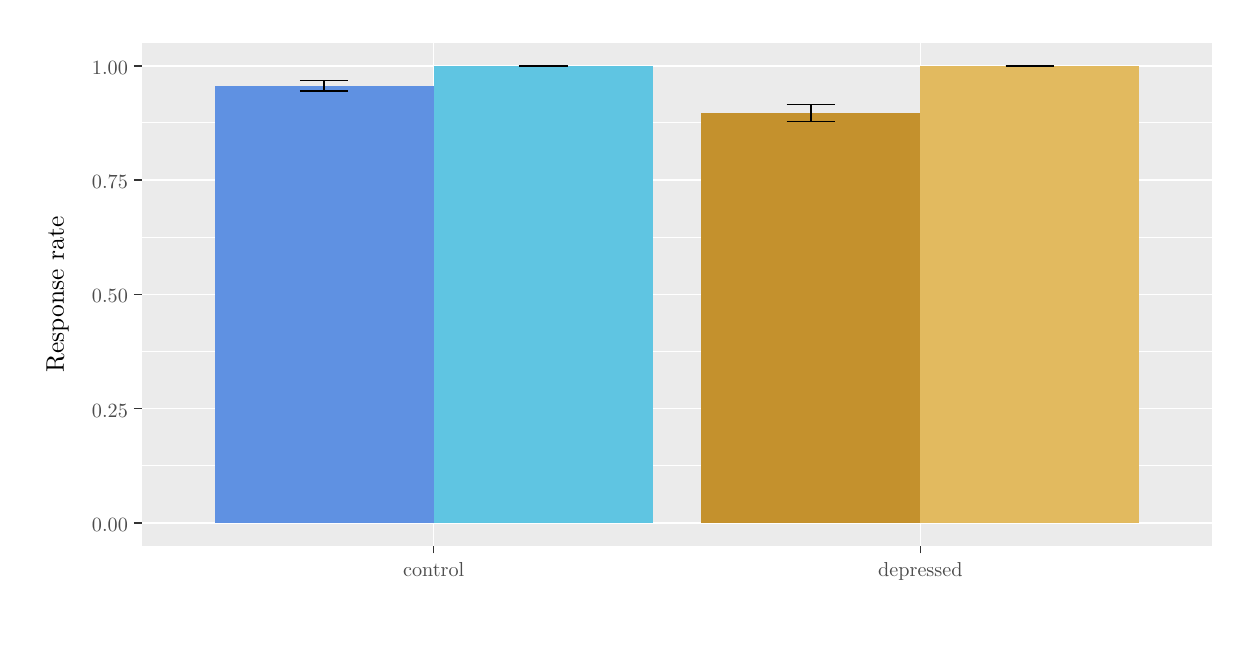
\begin{tikzpicture}[x=1pt,y=1pt]
\definecolor{fillColor}{RGB}{255,255,255}
\path[use as bounding box,fill=fillColor,fill opacity=0.00] (0,0) rectangle (433.62,216.81);
\begin{scope}
\path[clip] (  0.00,  0.00) rectangle (433.62,216.81);
\definecolor{drawColor}{RGB}{255,255,255}
\definecolor{fillColor}{RGB}{255,255,255}

\path[draw=drawColor,line width= 0.6pt,line join=round,line cap=round,fill=fillColor] (  0.00,  0.00) rectangle (433.62,216.81);
\end{scope}
\begin{scope}
\path[clip] ( 41.17, 29.59) rectangle (428.12,211.31);
\definecolor{fillColor}{gray}{0.92}

\path[fill=fillColor] ( 41.17, 29.59) rectangle (428.12,211.31);
\definecolor{drawColor}{RGB}{255,255,255}

\path[draw=drawColor,line width= 0.3pt,line join=round] ( 41.17, 58.50) --
	(428.12, 58.50);

\path[draw=drawColor,line width= 0.3pt,line join=round] ( 41.17, 99.80) --
	(428.12, 99.80);

\path[draw=drawColor,line width= 0.3pt,line join=round] ( 41.17,141.10) --
	(428.12,141.10);

\path[draw=drawColor,line width= 0.3pt,line join=round] ( 41.17,182.40) --
	(428.12,182.40);

\path[draw=drawColor,line width= 0.6pt,line join=round] ( 41.17, 37.85) --
	(428.12, 37.85);

\path[draw=drawColor,line width= 0.6pt,line join=round] ( 41.17, 79.15) --
	(428.12, 79.15);

\path[draw=drawColor,line width= 0.6pt,line join=round] ( 41.17,120.45) --
	(428.12,120.45);

\path[draw=drawColor,line width= 0.6pt,line join=round] ( 41.17,161.75) --
	(428.12,161.75);

\path[draw=drawColor,line width= 0.6pt,line join=round] ( 41.17,203.05) --
	(428.12,203.05);

\path[draw=drawColor,line width= 0.6pt,line join=round] (146.70, 29.59) --
	(146.70,211.31);

\path[draw=drawColor,line width= 0.6pt,line join=round] (322.59, 29.59) --
	(322.59,211.31);
\definecolor{fillColor}{RGB}{95,197,226}

\path[fill=fillColor] (146.70, 37.85) rectangle (225.85,203.05);
\definecolor{fillColor}{RGB}{95,145,226}

\path[fill=fillColor] ( 67.56, 37.85) rectangle (146.70,195.75);
\definecolor{fillColor}{RGB}{226,186,95}

\path[fill=fillColor] (322.59, 37.85) rectangle (401.74,203.05);
\definecolor{fillColor}{RGB}{196,145,45}

\path[fill=fillColor] (243.44, 37.85) rectangle (322.59,185.98);
\definecolor{drawColor}{RGB}{0,0,0}

\path[draw=drawColor,line width= 0.6pt,line join=round] (177.48,203.05) --
	(195.07,203.05);

\path[draw=drawColor,line width= 0.6pt,line join=round] (186.28,203.05) --
	(186.28,203.05);

\path[draw=drawColor,line width= 0.6pt,line join=round] (177.48,203.05) --
	(195.07,203.05);

\path[draw=drawColor,line width= 0.6pt,line join=round] ( 98.34,197.68) --
	(115.92,197.68);

\path[draw=drawColor,line width= 0.6pt,line join=round] (107.13,197.68) --
	(107.13,193.83);

\path[draw=drawColor,line width= 0.6pt,line join=round] ( 98.34,193.83) --
	(115.92,193.83);

\path[draw=drawColor,line width= 0.6pt,line join=round] (353.37,203.05) --
	(370.96,203.05);

\path[draw=drawColor,line width= 0.6pt,line join=round] (362.16,203.05) --
	(362.16,203.05);

\path[draw=drawColor,line width= 0.6pt,line join=round] (353.37,203.05) --
	(370.96,203.05);

\path[draw=drawColor,line width= 0.6pt,line join=round] (274.22,189.08) --
	(291.81,189.08);

\path[draw=drawColor,line width= 0.6pt,line join=round] (283.01,189.08) --
	(283.01,182.88);

\path[draw=drawColor,line width= 0.6pt,line join=round] (274.22,182.88) --
	(291.81,182.88);
\end{scope}
\begin{scope}
\path[clip] (  0.00,  0.00) rectangle (433.62,216.81);
\definecolor{drawColor}{gray}{0.30}

\node[text=drawColor,anchor=base east,inner sep=0pt, outer sep=0pt, scale=  0.73] at ( 36.22, 34.82) {0.00};

\node[text=drawColor,anchor=base east,inner sep=0pt, outer sep=0pt, scale=  0.73] at ( 36.22, 76.12) {0.25};

\node[text=drawColor,anchor=base east,inner sep=0pt, outer sep=0pt, scale=  0.73] at ( 36.22,117.42) {0.50};

\node[text=drawColor,anchor=base east,inner sep=0pt, outer sep=0pt, scale=  0.73] at ( 36.22,158.72) {0.75};

\node[text=drawColor,anchor=base east,inner sep=0pt, outer sep=0pt, scale=  0.73] at ( 36.22,200.02) {1.00};
\end{scope}
\begin{scope}
\path[clip] (  0.00,  0.00) rectangle (433.62,216.81);
\definecolor{drawColor}{gray}{0.20}

\path[draw=drawColor,line width= 0.6pt,line join=round] ( 38.42, 37.85) --
	( 41.17, 37.85);

\path[draw=drawColor,line width= 0.6pt,line join=round] ( 38.42, 79.15) --
	( 41.17, 79.15);

\path[draw=drawColor,line width= 0.6pt,line join=round] ( 38.42,120.45) --
	( 41.17,120.45);

\path[draw=drawColor,line width= 0.6pt,line join=round] ( 38.42,161.75) --
	( 41.17,161.75);

\path[draw=drawColor,line width= 0.6pt,line join=round] ( 38.42,203.05) --
	( 41.17,203.05);
\end{scope}
\begin{scope}
\path[clip] (  0.00,  0.00) rectangle (433.62,216.81);
\definecolor{drawColor}{gray}{0.20}

\path[draw=drawColor,line width= 0.6pt,line join=round] (146.70, 26.84) --
	(146.70, 29.59);

\path[draw=drawColor,line width= 0.6pt,line join=round] (322.59, 26.84) --
	(322.59, 29.59);
\end{scope}
\begin{scope}
\path[clip] (  0.00,  0.00) rectangle (433.62,216.81);
\definecolor{drawColor}{gray}{0.30}

\node[text=drawColor,anchor=base,inner sep=0pt, outer sep=0pt, scale=  0.73] at (146.70, 18.58) {control};

\node[text=drawColor,anchor=base,inner sep=0pt, outer sep=0pt, scale=  0.73] at (322.59, 18.58) {depressed};
\end{scope}
\begin{scope}
\path[clip] (  0.00,  0.00) rectangle (433.62,216.81);
\definecolor{drawColor}{RGB}{0,0,0}

\node[text=drawColor,rotate= 90.00,anchor=base,inner sep=0pt, outer sep=0pt, scale=  0.92] at ( 13.08,120.45) {Response rate};
\end{scope}
\end{tikzpicture}
